\section{\acrshort{ldr}}

Every \acrshort{lrp} needs to find a balance between the amount of privacy it provides, how close it is to the route cost optimum and how well it performs. The lightning routing triangle of success \cite{trampoline_routing_slides}, depicted here by figure \ref{fig:triangle}, portrays this balance for various routing protocols.

\begin{figure}[H]
\begin{center}
   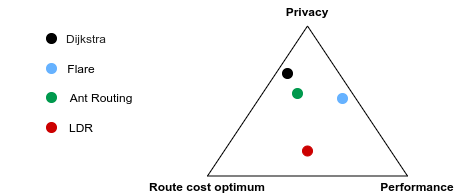
\includegraphics[width=0.9\linewidth]{images/triangle_paper.png}
  \caption{Lightning Routing Triangle of Success}
  \label{fig:triangle}
  \end{center}
\end{figure}

Because the current Dijkstra's shortest path algorithm based routing scheme prioritizes privacy and route cost optimization over performance its dot representation will appear in the left side of the triangle. The other routing protocols presented in section \ref{sec:background} make design decisions that place them in other places of the triangle, for example, Flare prioritizes performance at the cost of less cost-optimal routes, placing it in the right side of the triangle. \\
\acrshort{ldr} focuses on route costs and performance to the detriment of privacy, a compromise that is represented by its position at the bottom of the triangle. The reason behind this compromise is the fact that \acrshort{ldr} doesn't implement source routing and, instead of having the payer calculating the entire routing path, distributes this job and assigns it to the nodes that constitute the path, leaking the identity of the payee along the way. Nodes that constitute the path will use the locally stored information about the network to find the best next hop to reach the payee, an idea similar to the one behind distance-vector routing, studied in section \ref{ssec:distancevectorrouting}. Distributing the route-finding workload and leveraging the local knowledge of the network allows \acrshort{ldr} to increase performance while still keeping a small route cost. \\
\acrshort{ldr} operates over a dedicated peer-to-peer messaging network where nodes share routing info and dispatch routing requests. To find payment routes, nodes will use the information they have available in their routing tables, frequently sharing it and updating it accordingly so to follow the dynamic nature of the network. Instead of maintaining routing tables that associate destination nodes with their distance in the network and the next hop needed to get there like in most distance-vector routing protocols, \acrshort{ldr} associates destinations to the maximum volume that a payment can have to be successful in paying to that destination node and the next hop to be chosen in order to get there. It can be thought of as a \textit{capacity-vector} routing protocol, a distributed, one-path solution to a flow problem. \\
The success of the suggested protocol is a function of how well the routing tables in a given node can approximate the maximum capacity for a payment to a payee node, this will itself depend on how successful nodes are in sharing with the network the balances of their own channels. \\
Figure \ref{fig:architecture} details a complete view of the various components of an \acrshort{ldr} node and how they interact with each other and the external networks.

\begin{figure}[H]
\begin{center}
  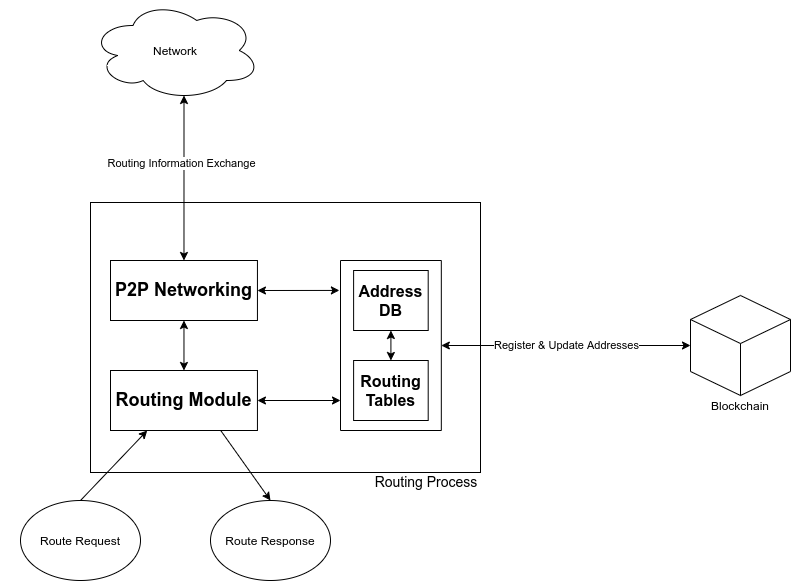
\includegraphics[width=0.9\linewidth]{images/architecture.png}
  \caption{\acrshort{ldr} Architecture}
  \label{fig:architecture}
  \end{center}
\end{figure}

The address database contains information about every known registered address. Every lightning network node is allowed to register an address and only registered nodes are allowed to be a part of the \acrshort{ldr} network, accessed through the P2P networking module. \\
The routing tables module contains the routing information associated with every registered address and the corresponding subnetworks, it periodically shares, receives and updates its information with new information from neighbouring nodes. \\
The routing module is responsible for receiving, processing and forwarding or responding to route requests made to the node. Requests might originate from a user needing a payment path to a node he's paying to or from a neighbouring node forwarding a third party route request.

\subsection{Component Analysis}
\label{ssec:component_analysis}
\subsubsection{Address DB}

The goal of the address database is to keep an updated list of every valid \acrshort{ldr} address so the node can always confirm the authenticity of the node he is communicating with. When a new address is registered it is also associated with a public key that can, from that point forward, be used to verify signatures that could only be constructed by the node that registered the address associated with that public key.\\
To populate the database with every valid address the entire set of blockchain transactions are analyzed and validated according to the rules specified in section \ref{sssec:blockchain_sync}. Locally validating the registration of every address allows for the existence of a decentralized and eventually consistent address database which does not rely on a central authority for its own existence and maintenance. Although it would be simpler to use a centralized scheme to maintain an address database this solution maintains the inherent decentralization of the bitcoin protocol stack while also offering a bigger degree of security against all types of attacks that only a centralized solution would be vulnerable against. \\
The rules designed to validate the address registrations present in special OP\_RETURN blockchain transactions were designed to promote the health of the network. By assigning new addresses based on the addresses of the neighbourhood a relation between a nodes address and their position in the network graph is created. This address assigning method takes inspiration from the centralized version, consisting of the assignment of blocks of addresses by a centralized authority and, like its centralized version, promotes the existence of routing tables with a smaller number of entries who can be grouped together by the use of address masking, much like what it is already done today by the routing tables implemented to support the distance-vector routing protocols mentioned in section \ref{ssec:distancevectorrouting}. Smaller routing tables decrease the computing and storage needs of each node while also reducing the amount of bandwidth needed to share them.

\subsubsection{Routing Tables}
\label{sssec:routing_tables}

Routing tables hold the information that allows nodes to make their routing decisions. They maintain up to date information on every known payment destination and the best next hop that should be taken in order to reach them. The "best next hop" for a certain payment destination is defined as being the hop with the lowest fee from the group of next hops for that destination where the maximum volume allowed is bigger than the payment's volume. \\
Throughout the rest of this section, we will use the example network represented by figure \ref{fig:networkabcd} to understand how nodes share and update their routing tables.\\

\begin{figure}[H]
\begin{center}
  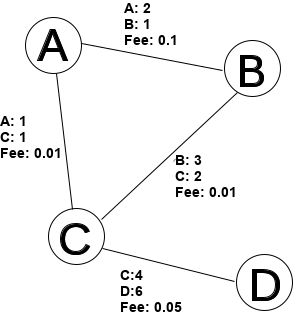
\includegraphics[width=0.6\linewidth]{images/networkabcd_cap.png}
  \caption{Example Lightning Network. Inspired by \cite{distance_vector}.}
  \label{fig:networkabcd}
  \end{center}
\end{figure}

Nodes populate their initial routing table with the information they have locally available, this is, the information about the distribution of the funds in the channels in which they take part. These entries are never removed from local memory and should always reflect the state of the underlying payment channels. Table \ref{table:routing_table_initial_a} and represents the initial \acrshort{ldr} routing tables of node A.

\begin{table}[H]
\begin{tabular}{|l|l|l|l|}
\hline
\rowcolor[HTML]{C0C0C0} 
Destination & Max. Volume   & Fee   & Next Hop \\ \hline
B           & 2             & 0.1   & B       \\ \hline
C           & 1             & 0.01  & C       \\ \hline
\end{tabular}
\caption{Node A's initial routing table}
\label{table:routing_table_initial_a}
\end{table}

Nodes will then start sharing routing gossip messages containing part or the entirety of their own routing tables. To sharing more about a node's neighbourhood than needed, information about the next hops is omitted from the gossip messages. Table \ref{table:routing_gossip} is an example of what a gossip message based on Node A's initial routing table (\ref{table:routing_table_initial_a}) might look like.

\begin{table}[H]
\begin{tabular}{|l|l|l|}
\hline
\rowcolor[HTML]{C0C0C0} 
Destination & Max. Volume   & Fee   \\ \hline
B           & 2             & 0.1   \\ \hline
C           & 1             & 0.01  \\ \hline
\end{tabular}
\label{table:routing_gossip}
\end{table}

On receiving a routing gossip message nodes update their routing tables with the new information accordingly. \\
Let $M$ be the updated maximum volume associated with the destination $D$, $F$ the associated fee, $O$ the outbound capacity of the channel associated with the node $N$ who sent the gossip message and $O\_F$ that channel's payment fee. Now let $V = min(M, O)$: \\

\begin{enumerate}

\item If there are no entries under the destination $D$ the ($D$, $V$, $F$ + $O\_F$, $N$) entry should be added to the routing table.
\item If there are only entries for the destination $D$ whose next hop is not $N$ the ($D$, $V$, $F$, $N$) entry should be added if $V$ is higher than the maximum volume of all those entries or if it is as high as the maximum volume entry but advertises a smaller payment fee but can be always added if the node decides to do so.
\item If there is already an entry for the destination $D$ whose next hop is $N$ the ($D$, $V$, $F$, $N$) entry should update that entry.

\end{enumerate}

From the second rule follows that the amount of locally stored entries for each destination is customizable, allowing each node operator to tailor it according to his memory requirements.\\
After enough routing gossip messages are shared the network will eventually reach a steady-state where new gossip messages do not change any of the information already available in the locally stored routing tables. Table \ref{table:routing_table_steady_a} represent the routing tables for node A after the steady-state is reached.

\begin{table}[H]
\begin{tabular}{|l|l|l|l|}
\hline
\rowcolor[HTML]{C0C0C0} 
Destination & Max. Volume   & Fee   & Next Hop \\ \hline
B           & 2             & 0.1   & B       \\ \hline
C           & 2             & 0.11  & B       \\ \hline
C           & 1             & 0.01  & C       \\ \hline
D           & 2             & 0.16  & B       \\ \hline
\end{tabular}
\caption{Node A's steady-state routing table}
\label{table:routing_table_steady_a}
\end{table}

After the steady-state is reached the network must be able to adapt to the frequent changes in the distribution of the funds in the payment channels.\\
For example, if A sends 1 BTC to B, making their shared their channel state become (A: 1, B: 2), both nodes will reevaluate their routing tables focusing on the entries in which the next hop is the neighbour that shares the channel in which the payment took place. These reevaluation yields routing table \ref{table:routing_table_payment_a}.

\begin{table}[H]
\begin{tabular}{|l|l|l|l|}
\hline
\rowcolor[HTML]{C0C0C0} 
Destination & Max. Volume   & Fee   & Next Hop \\ \hline
B           & 1             & 0.1   & B       \\ \hline
B           & 1             & 0.02  & B         \\ \hline
C           & 1             & 0.01  & C       \\ \hline
D           & 1             & 0.06  & C       \\ \hline
\end{tabular}
\caption{Node A's routing table after payment}
\label{table:routing_table_payment_a}
\end{table}

The information present in these updated routing tables is then shared through gossip messages with A's and B's neighbours and eventually propagated through the entire network until another steady-state is reached. Routing tables \ref{table:routing_table_steady_a_2} represent node A's table at this second steady-state.

\begin{table}[H]
\begin{tabular}{|l|l|l|l|}
\hline
\rowcolor[HTML]{C0C0C0} 
Destination & Max. Volume   & Fee   & Next Hop \\ \hline
B           & 1             & 0.1   & B       \\ \hline
C           & 1             & 0.11  & B       \\ \hline
C           & 1             & 0.01  & C       \\ \hline
D           & 1             & 0.16  & C       \\ \hline
\end{tabular}
\caption{Node A's second steady-state routing table}
\label{table:routing_table_steady_a_2}
\end{table}

Routing gossip messages must be frequently exchanged between neighbours so that the dynamic nature of the network, especially the frequently updated outbound capacities, can be correctly reflected on the state of a node's routing table. However, allowing the exchange of this type of information between neighbouring nodes compromises privacy by giving neighbouring nodes access to information that would otherwise be private, a compromise made in exchange for the increase in performance given by the augmented knowledge each node has on the network.

\subsubsection{P2P Networking Module}

The peer-to-peer networking module is the gateway between the other components of \acrshort{ldr} and the rest of the nodes in the network. It provides communication with other nodes while also authenticating them, this is, making sure communications only happens between nodes with valid \acrshort{ldr} addresses.

\subsubsection{Routing Module}

The routing module has two main functions, it creates route requests if a new payment route is requested by the user or forwards route requests that were relayed by a neighbour. \\
When a user wants to find a new route for a lightning payment a new route request is created. The routing module finds the best next hop to send the request to and waits for an answer from the destination node or a time-out. If the request reaches the destination node it means it travelled, hop-by-hop, through the payment path, registering the path along the way. This path is then sent back to the user who uses it to build his lightning payment. \\
When a node receives a routing request it starts by checking if the request's destination is itself, if it is the node returns the request to its sender, if it isn't the node forwards the request to the best next hop for that request's destination, adding itself to the payment path that is being collected by the route request along the way.